\documentclass[a4paper,11pt]{article}
%Przydatne paczki:
\usepackage{amssymb}
\usepackage{amsthm}
\usepackage{amsmath}
\usepackage[colorinlistoftodos]{todonotes}
\usepackage[colorlinks=true, allcolors=blue]{hyperref}
%Definicja kodowania i języka:
\usepackage[polish]{babel}
\usepackage[MeX]{polski}
\usepackage[utf8]{inputenc}
\usepackage[T1]{fontenc}
%Paczki dodane w drodze pisania:
\usepackage{graphicx}
\usepackage{anysize}
\selectlanguage{polish}
\usepackage{tabularx}
\usepackage[export]{adjustbox}
\usepackage{listings}
\usepackage{float}
\usepackage{fancyhdr}

%Nagłówek:
\pagestyle{fancy}
\fancyhead{}
\fancyhead[L]{\small{\bfseries \thepage}}
\fancyfoot[L, C, R] {}
\fancyhead[C]{\small{\bfseries Dokumentacja projektu "Reflekto"}}
\renewcommand{\headrulewidth}{0.8pt}

%\marginsize{left}{right}{top}{bottom}
\marginsize{2.5cm}{2.5cm}{2.5cm}{2.5cm}

\begin{document}

\title{Dokumentacja projektu \\ \textbf{,,Reflekto'' } }
\author{Michał Kwiecień \\ Michał Wójcik}
%skomentować żeby nie było daty
%\date{\vspace{-5ex}}
\maketitle

\begin{abstract}
Dokumentacja projektu inteligentnego lustra w konwencji IoT komunikującego się ze smartfonem z użyciem interfejsu Bluetooth Low Energy. Projekt powstał na potrzeby konkursu Nordic Semiconductor Student Contest. 
\end{abstract}

\begin{figure}
	
\includegraphics[width=0.3\textwidth,center]{logo_nordic.png}
\end{figure}

\cleardoublepage
\tableofcontents
\clearpage

\section{Ogólny opis projektu}

Założeniem projektu jest stworzenie inteligentnego lustra, które podczas wykonywania codziennych czynności, umożliwi podgląd najświeższych i spersonalizowanych informacji. Informacje te zostaną wyświetlone na ekranie umieszczonym za lustrem weneckim, dzięki czemu będą widoczne jednocześnie obok odbicia. 

Działanie lustra opiera się na przekazaniu danych poprzez moduł Bluetooth ze smartfona do modułu nRF52 i umieszczeniu ich na podłączonym ekranie. Aktywacja lustra nastąpi w momencie zbliżenia się do niego użytkownika. Z lustra może korzystać wielu użytkowników, gdyż każdorazowo przesyłane są indywidualne dane dla każdego z nich. 

W celu wygenerowania danych stworzona została dedykowana aplikacja dla systemu iOS. Po wstępnej konfiguracji umożliwi ona zautomatyzowanie procesu i przesyłanie wiadomości w tle bez późniejszych ingerencji użytkownika.


\section{Prezentacja działania}

Kiedy lustro nie jest w bliskim zasięgu jednego ze sparowanych telefonów, wyświetlana jest godzina lub pozostaje wyłączone w zależności od ustawień (Rys. \ref{lustro_off})

\begin{figure}[H]
	
\includegraphics[width=0.6\textwidth,center]{mirror_off.png}
	\caption {Lustro w stanie wyłączonym}
	\label{lustro_off}
\end{figure}

W momencie zbliżenia się użytkownika, następuje transmisja danych i wyświetlenie aktualnych wiadomości (Rys. \ref{lustro_on}).

\begin{figure}[H]
	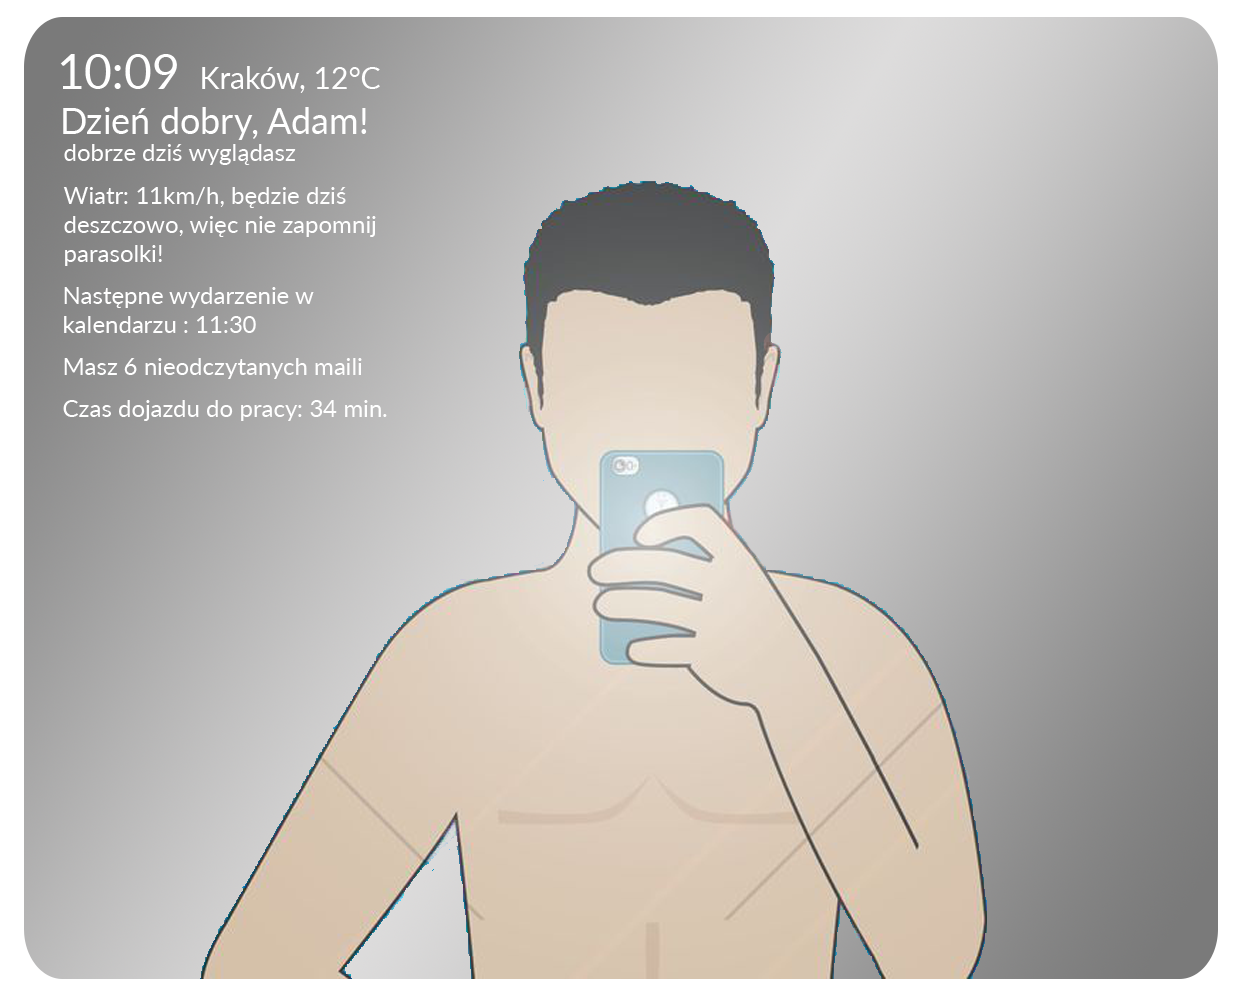
\includegraphics[width=0.6\textwidth,center]{mirror_on.png}
	\caption {Lustro w stanie aktywnym}
	\label{lustro_on}
\end{figure}

\section{Planowane możliwości personalizacji}
\begin{figure}[H]
	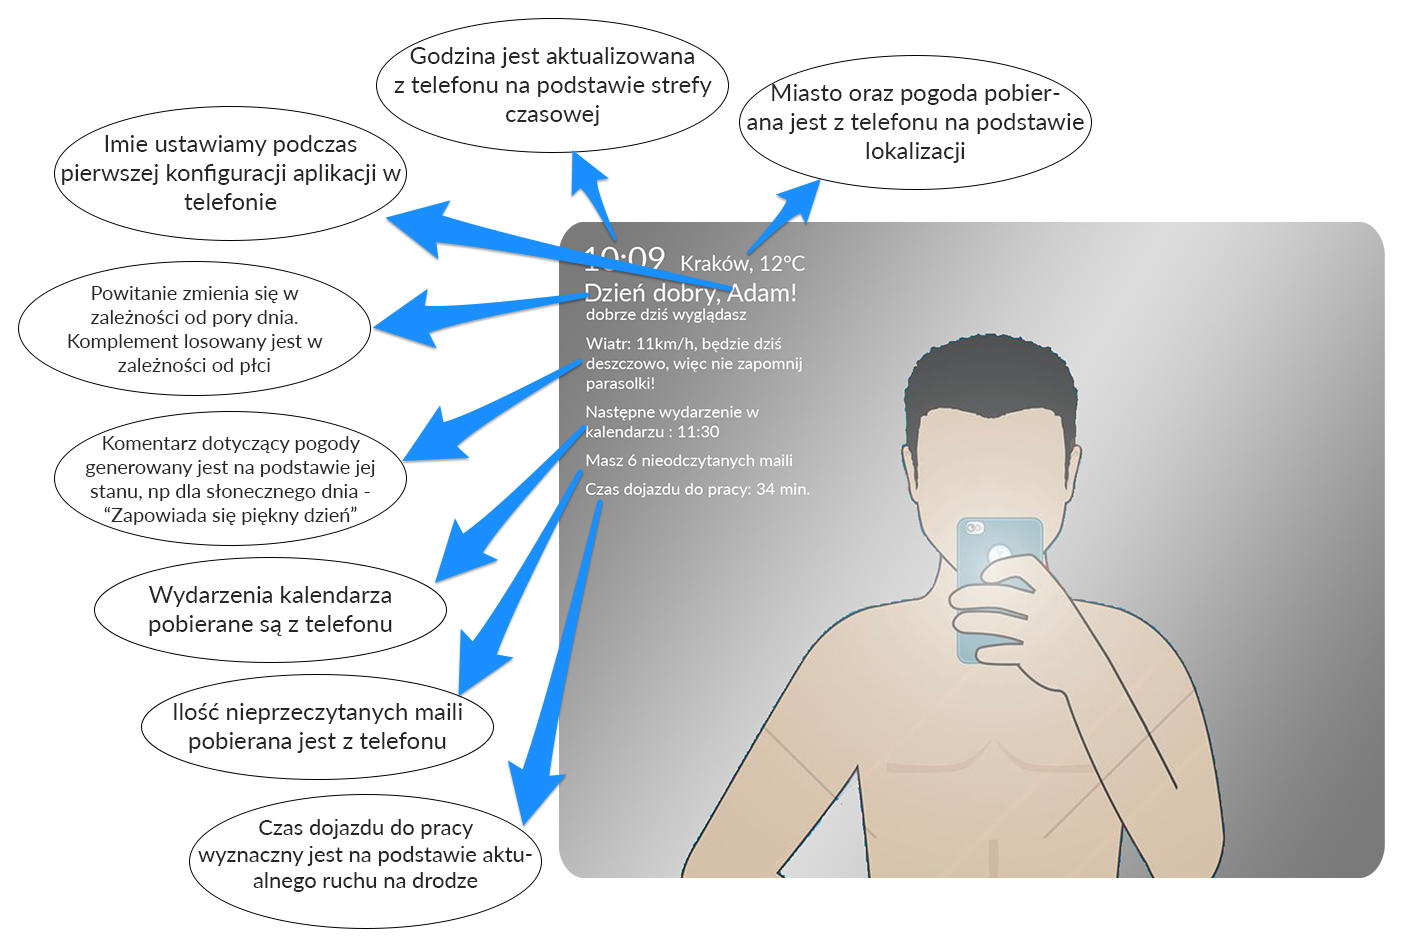
\includegraphics[width=0.9\textwidth,center]{dymki_kreski.png}
	\caption {Proponowane możlwości personalizacji}
	\label{lustro_on}
\end{figure}

\section{Opis aplikacji systemu nRF52 }

\section{Opis aplikacji systemu iOS}



	
\end{document}